
\section{Client Overview}
\label{sec:client_des}

\begin{figure*}[!t]
   \centering
      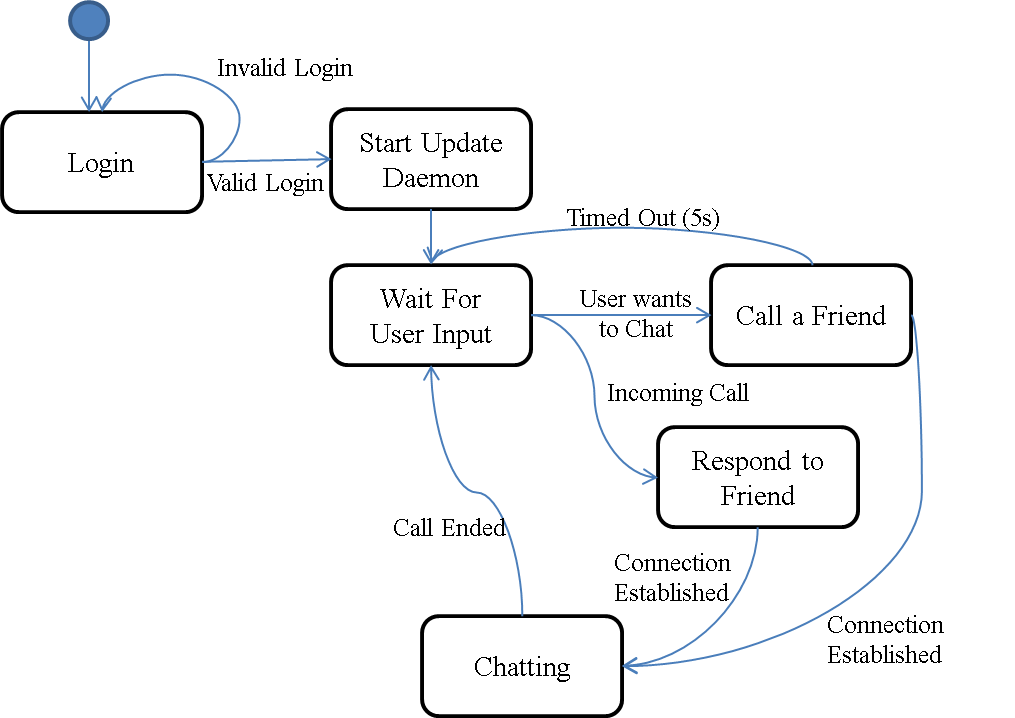
\includegraphics[width=0.8\textwidth]{pics/Client_StateDiagram}
   \caption{Client State Diagram demonstrating the general flow on the client-side.}
\label{fig:client_state_diag}
\end{figure*}

The client application is the core of the voice chatting system.  It initiates all
the communication with the server in order to receive the user's personal 
information which includes a friends list. For purposes of this paper, a friend
is one whom appears on the list of people a user can call. The application currently
does not support the ability for users to add friends during run-time.  Once the 
user logs into the server,
the client has free roam to make outgoing calls or answer incoming calls.  This
application only supports one-to-one chatting with a notification system that 
indicates when a friend is calling while the user is chatting with another client.  

The client-side of the system handles all the audio transmission between clients
as well as manages the setup and teardown of the transport protocol used to
communicate between two clients.  Each client is fitted with a transport protocol
object that handles all the layer three calls which send and receive data between
two clients using sockets.  The specific transport layer protocol is determined
upon loading the application by the user where DCCP, UDP, and TCP are the three
options. Each client is capable of calling friends as well as accepting calls from
other clients.  This requires a \textit{server} and \textit{client} model present
on each client's machine in order to monitor a socket for incoming calls as well
as open a new socket for outgoing calls.  Fig.~\ref{fig:client_state_diag} gives 
a state diagram representation of the client-side system.


The client communicates with the server once upon logging into the system and again
every time a client wants to call a friend.  When making an outgoing call,
the client asks the server for the hostname and port number of the friend he or
she wants to call.  This information is relayed back to the requestor which is then
used to directly call the friend of interest.  Since all communication with the
server contains important information about how to contact others within the 
network, the connection needs to be reliable; therefore, TCP is used for all 
communication between the clients and the server. Additionally, a seperate thread
is started immediately after logging into the server that handles receiving
periodic messages from the server which indicate any changes in the user's friends'
statuses. 


\subsection{Transport Layer Abstraction}
\label{subsec:transport_abs}

The main feature of this voice chatting application is its ability to easily 
swap in and out different transport layer protocols.  Essentially, this application
is a framework for testing the behavior of transport layer protocols with an
audio streaming application.  The abstraction was designed using the concept of
polymorphism.  Basically, a class called \textit{TransProtocol} was constructed
with several virtual functions that inhereting children must implement, i.e. DCCP,
TCP, and UDP.  These include the following:

\begin{itemize}
   \item{initMaster(uint16\_t)}
   \item{initSlave(char *, uint16\_t)}
   \item{sendPacket(void *, size\_t)}
   \item{recvPacket(void *, size\_t, int flags)}
   \item{getCallerID()}
   \item{ignoreCaller()}
   \item{answerCall()}
   \item{endCall()}
\end{itemize}

The above functions need to be implemented individually according to the specific
transport layer protocol.  For example, DCCP and TCP are connection-oriented and
need to setup a connection between two computers initially before any data packets 
can be transmitted whereas UDP connections open a socket and wait for 
whomever decides to send data its way.  The initialization steps for each of the
different transport layer protocols occur in the functions \textit{initMaster} and
\textit{initSlave}.  These two functions differ in the way the sockets are handled.

For the \textit{initMaster} function, the socket is bound to a randomly selected 
port in the same manner as the server does in a traditional server-client TCP model.
This port is then configured to listen for incoming requests. 
Before any clients can call this user, the port number needs to be reported to
the central server which saves it to a database. This port is continuously 
monitored by the client to notify the user of any incoming calls.  When an incoming
call is detected, the client machine accepts the call and extracts the caller's 
identification from the first packet to determine who the caller is using the 
\textit{getCallerID} function.  At this point, the user is notified when an 
incoming request has been received and is given the option to accept or decline
the call.  The appropriate action is taken based on the users response.

The \textit{initSlave} function is used when a client wants to make an outgoing
call to a friend.  For this to occur, the client machine requests from the central 
server the hostname and port number of the friend he or she wants to call 
identified by the user identification number.  After retrieving the proper contact 
information from the central server, \textit{initSlave} opens a socket to 
communicate with the friend.  Similar to the \textit{initMaster} function, if the
callee accepts the users call, then the chatting state will be entered and audio
capturing and playback will begin while being transferred across the transport
layer protocol of choice.

To handle processing the audio transmission and incoming chatting requests, the
main application was multi-threaded using boost threads.  Basically, the main
application thread handles the incoming requests and parses through the first
incoming request packets to identify who the caller is.  Once a connection
is established between two clients and the callee accepts the call, a chatting
thread is spawned that handles the audio capturing and playback along with the 
packet construction and transmission.  Within the chatting thread, there is an
audio playback thread started, which is discussed in the next section.


\subsection{Audio Processing}
\label{subsec:audio_proc}

Audio transmission was handled in the simplest possible manner.  The ALSA libraries
were used to capture and playback the raw audio from the microphone on each of the 
client's machines.  The ALSA libraries were used because of their simplicity and
built-in linux functionality.   

The audio was captured at 8,000 bytes per second on 2 channels.  In a 
single packet, 1,400 bytes are transmitted.  The capture and transmission of audio 
data occurs in the main chatting thread while the playback of the received audio 
packets occurr in a seperate thread.  This thread is dedicated to reading from
a buffer that contains received audio packets.  To reduce the latency 
introduced by transmitting in real-time over a network, a minimum buffer size
threshold was set to 5 packets.

